% batch_server: threads, the shared lock, and the wait chain that sets each
% round's length. Standalone; build with
%   pdflatex batch_server.tex
% and include the PDF with 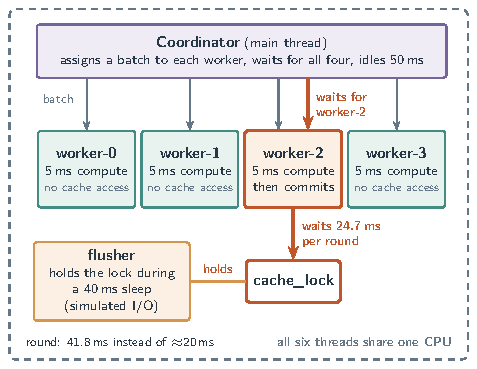
\includegraphics[width=\columnwidth]{batch_server}.
% Colours follow traceassist_pipeline.tex. A thread-and-lock diagram, not a
% timeline: the averages alone do not fix the ordering within a round.
\documentclass[tikz,border=1.5mm]{standalone}
\usepackage[T1]{fontenc}
\usepackage{lmodern}
\usetikzlibrary{arrows.meta,positioning,calc}

\definecolor{ink}{HTML}{273746}
\definecolor{line}{HTML}{657786}
\definecolor{purple}{HTML}{75649C}
\definecolor{teal}{HTML}{428C83}
\definecolor{orange}{HTML}{D5954C}
\definecolor{chain}{HTML}{C2562B}
\definecolor{greenfill}{HTML}{E8F3F0}
\definecolor{lavender}{HTML}{F0ECF5}
\definecolor{orangefill}{HTML}{FBF0E3}

\newcommand{\hd}[1]{{\bfseries\fontsize{7.5}{9}\selectfont #1}}

\begin{document}
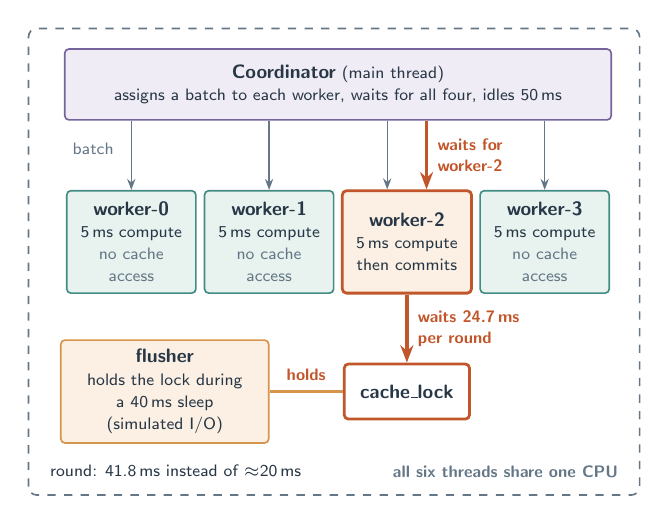
\begin{tikzpicture}[
  font=\sffamily\fontsize{6.5}{8}\selectfont, text=ink,
  thread/.style={draw, rounded corners=1.5pt, align=center, inner sep=1.2mm,
                 line width=.6pt},
  worker/.style={thread, draw=teal, fill=greenfill, text width=14.6mm, minimum height=13mm, inner sep=.9mm},
  note/.style={font=\sffamily\fontsize{5.8}{7}\selectfont, text=line},
  plain/.style={draw=line, line width=.5pt, -{Stealth[length=1.4mm]}},
  waits/.style={draw=chain, line width=1.3pt, -{Stealth[length=2.2mm]}},
  lbl/.style={font=\sffamily\fontsize{6}{7.5}\selectfont, text=line},
  chainlbl/.style={font=\sffamily\bfseries\fontsize{6.2}{7.5}\selectfont, text=chain}]

% ---- threads -------------------------------------------------------------
\node[thread, draw=purple, fill=lavender, text width=67mm, minimum height=9mm] (co) at (0,0)
  {\hd{Coordinator} (main thread)\\ assigns a batch to each worker, waits for all four, idles 50\,ms};

\node[worker] (w0) at (-26.25mm,-20mm) {\hd{worker-0}\\ 5\,ms compute\\ {\fontsize{5.8}{7}\selectfont\color{line}no cache access}};
\node[worker] (w1) at (-8.75mm,-20mm)  {\hd{worker-1}\\ 5\,ms compute\\ {\fontsize{5.8}{7}\selectfont\color{line}no cache access}};
\node[worker, draw=chain, fill=orangefill, line width=1pt] (w2) at (8.75mm,-20mm)
  {\hd{worker-2}\\ 5\,ms compute\\ then commits}; 
\node[worker] (w3) at (26.25mm,-20mm) {\hd{worker-3}\\ 5\,ms compute\\ {\fontsize{5.8}{7}\selectfont\color{line}no cache access}};

\node[thread, draw=chain, fill=white, line width=1pt, text width=13.5mm, minimum height=7mm]
  (lock) at (8.75mm,-39mm) {\hd{cache\_lock}};
\node[thread, draw=orange, fill=orangefill, text width=24mm, minimum height=10mm]
  (fl) at (-22mm,-39mm)
  {\hd{flusher}\\ holds the lock during\\ a 40\,ms sleep\\ (simulated I/O)};

% ---- work assignment (grey) ----------------------------------------------
\foreach \w in {w0,w1,w3} {
  \draw[plain] (co.south -| \w.north) -- (\w.north);
}
\draw[plain] ($(co.south -| w2.north)+(-2.5mm,0)$) -- ($(w2.north)+(-2.5mm,0)$);
\node[lbl, anchor=east] at ($(co.south -| w0.north)+(-1mm,-3.5mm)$) {batch};

% ---- the wait chain (highlighted) ----------------------------------------
\draw[waits] ($(co.south -| w2.north)+(2.5mm,0)$) -- node[chainlbl, right, align=left]
  {waits for\\ worker-2} ($(w2.north)+(2.5mm,0)$);
\draw[waits] (w2.south) -- node[chainlbl, right, align=left]
  {waits 24.7\,ms\\ per round} (lock.north);
\draw[draw=orange, line width=1.3pt] (fl.east) -- node[lbl, above, text=chain,
  font=\sffamily\bfseries\fontsize{6.2}{7.5}\selectfont] {holds} (lock.west);

% ---- shared CPU and the result -------------------------------------------
\coordinate (sw) at ($(fl.south west)+(-4mm,-6.5mm)$);
\coordinate (ne) at ($(co.north east)+(3.5mm,2.5mm)$);
\draw[line, dashed, rounded corners=3pt, line width=.6pt] (sw) rectangle (ne);
\node[lbl, anchor=south east, font=\sffamily\bfseries\fontsize{6.2}{7.5}\selectfont]
  at ($(ne |- sw)+(-1.5mm,1mm)$) {all six threads share one CPU};
\node[lbl, anchor=south west, text=ink] at ($(sw)+(1.5mm,1mm)$)
  {round: 41.8\,ms instead of $\approx$20\,ms};

\end{tikzpicture}
\end{document}
